
As \emph{Redes Neurais Artificiais} (RNAs) são modelos computacionais inspirados na capacidade de processamento de informações do cérebro humano \cite{ref2:rojas}.\todo{Sugerir Haykin} De acordo com esta ideia, possuem unidades de processamento simples, denominadas \emph{neurônios artificiais}, dispostos em camadas interconectadas por ligações associadas a coeficientes numéricos, chamados \emph{pesos} []. As RNAs são capazes de aprenderem padrões complexos a partir dos dados e prever resultados para exemplos não conhecidos, o que demonstra a sua capacidade de generalização [].

% Neurônio Artificial

O neurônio artificial é a unidade fundamental na construção de RNAs, tendo sido inspirado no seu análogo biológico. Segundo Rosenblat \todo{citar},  existe um conjunto de $m$ entradas, equivalentes aos dendritos de um neurônio biológico, por onde os sinais são introduzidos. Associa-se um peso a cada entrada, representando a relevância referente a uma conexão sináptica. Há também o peso $w_0$, um termo de polarização criado com a intenção de estabelecer um limitar de ativação para cada neurônio. Este peso corresponde à entrada \emph{bias}, cujo valor é sempre unitário. Pode-se então definir um vetor de entradas $X = [+1, x_1, x_2, \ldots, x_m]$ e um vetor de pesos $W = [w_0, w_1, \ldots, w_m$]. As entradas e pesos são combinados por meio de uma função $\phi: \mathbbm{R}^{m+1} \rightarrow \mathbbm{R}$, que é geralmente a soma ponderada das entradas e pesos, conforme Eq. \ref{eq:somaPonderada}. Este modelo de neurônio encontra-se ilustrado na Figura \ref{img:neuronioArtificial}.

\begin{equation}
\phi(X,W) = \sum_{i =0}^m x_i \cdot w_i \label{eq:somaPonderada}
\end{equation}

\begin{figure}[h!]
	\centering
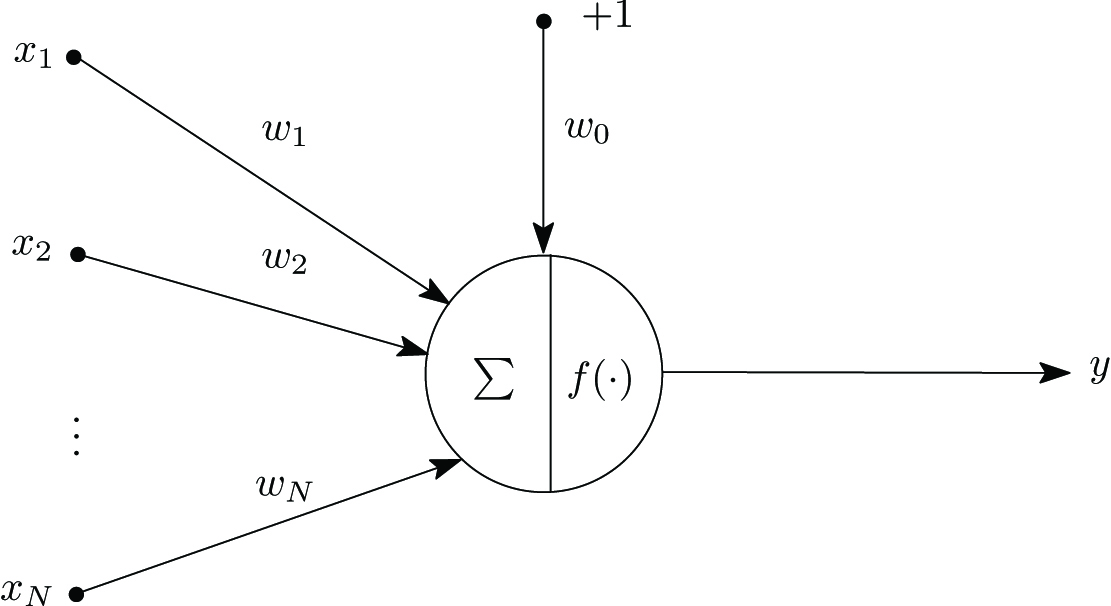
\includegraphics[width=0.6\textwidth]{./img/neuron}
\caption{Falta legenda!}\label{img:neuronioArtificial}
\end{figure}

A função $f$ é chamada de \emph{função de ativação} e fornece a resposta de um neurônio para uma dada entrada. Esta função é monotônica e contínua, podendo comumente ser as funções identidade, sigmóide hiperbólica, tangente hiperbólica, ou a retificada linear (ReLU). Estas funções encontram-se representadas na Figura X.

\missingfigure{Fazer a figurinha com as quatro funções de ativação.}

\begin{comment}
	\begin{figure}[h!]
		\centering
		\subfloat[Janela de tempo $w = 1$. \label{img:1ano}]{\includegraphics[width=0.5\linewidth]{./img/boxplot1ano}}
		\subfloat[Janela de tempo $w = 2$.\label{img:2anos}]{\includegraphics[width=0.5\linewidth]{./img/boxplot2anos}}\\
		\subfloat[Janela de tempo $w = 3$. \label{img:3anos}]{\includegraphics[width=0.5\linewidth]{./img/boxplot3anos}}
		\subfloat[Janela de tempo $w = 4$.\label{img:4anos}]{\includegraphics[width=0.5\linewidth]{./img/boxplot4anos}}
		\caption{Boxplot da medida \textit{F-score} das 4 técnicas de AM para as quatro janelas de tempo.}
	\end{figure}
\end{comment}

% Multilayer Perceptron
Neurônios artificiais têm uma capacidade computacional limitada, independentemente da função de ativação escolhida. No entanto, um conjunto de neurônios artificiais conectados na forma de uma rede -- \emph{rede neural artificial} -- adquirem a capacidade de resolver problemas de elevada complexidade \cite{Teresa:Livro}.


Disposição dos neurônios em camadas
Papel das camadas ocultas

\missingfigure{Figura com representação de RNA.}


% Paradigma supervisionado
%% Aprendizado sentido forward


% backpropagation




% Exemplos





 As redes do tipo \textit{Multilayer Perceptron} (MLP) pertencem à arquitetura \textit{feedforward} com múltiplas camadas divididas em: camada de entrada, uma ou mais camadas ocultas e camada de saída \cite{ref10:faceli}.

O algoritmo mais tradicional utilizado no processo de aprendizado (treinamento) das redes MLP é o algoritmo de retropropagação do erro ou \textit{backpropagation} \cite{ref11:teive}. Durante o treinamento a rede recebe atributos de entrada que são ponderados e combinados entre as camadas por meio dos neurônios por uma função matemática, chamada função de ativação, gerando ao final um valor de saída. Com base no resultado obtido, a próxima etapa consiste na correção dos pesos de cada neurônio que são ajustados proporcionalmente ao seu erro. Esse processo se repete até que seja alcançado um erro mínimo definido e o treinamento seja interrompido \cite{ref10:faceli,ref1:guedes,ref5:aguni}.

\newpage

As RNAs têm sido utilizadas para aplicações em diversas áreas como Geografia \cite{ref11:teive}, Biologia \cite{ref7:duarte}, Comunicação \cite{ref12:balieiro} e na área Industrial \cite{ref4:prego}. Muitos estudos utilizam as RNAs para classificação de dados, como \cite{ref1:guedes} e \cite{ref3:lima}, ou para previsão de informações como em \cite{ref7:duarte}. No processamento de imagens, as RNAs atuam principalmente em conjunto com as técnicas de Aprendizado Profundo ou \textit{Deep Learnig}.

\begin{itemize}
	\item Ideia
	\item Conceitos
	\begin{itemize}
		\item Camadas -- camada oculta
		\item Neurônios, pesos
		\item Funções de ativação
	\end{itemize}
	\item Aprendizado das RNAs
	\begin{itemize}
		\item Backpropagation
		\item Generalização -- aproximadora universal
	\end{itemize}
	\item Aplicações
\end{itemize}
